%Intro_Arduino_ComputerControl
\chapter{Introduction to the Arduino}

\objectives{
\item Explain how to use a prototyping board, including the identification of
which pins are electrically connected.
\item Demostrate proper soldering technique.
\item Describe the two primary functions included in every Arduino sketch, when
they are called, and what they do.
\item Compile and upload sketches to an Arduino.
\item Demonstrate the use of digital output on the Arduino by constructing 
several circuits involving blinking lights.
}

\review{
\item Voltage (electric potential).
\item Current.
\item Resistance.
\item Diodes and LEDs.
}

There are two ways in which we want our computers to communicate with our
physics experiments:
\begin{enumerate}
\item Have the computer control the experiment. For example, we could have the
computer turn on our apparatus, or turn it off. 
\item Have the experimental device provide data to the computer. The computer
can then record this data for later analysis.
\end{enumerate}
In both cases, we need something that goes between the
experimental measuring devices and the computer. These go-between pieces are
often called Data Acquisition (DAQ) boards. There are many different forms
of DAQs. They can cost anywhere from a few dollars to many thousands of
dollars.

In this lab, we will use a low cost DAQ, the plans for which the 
developers placed in the open-source world so that no one
would get royalties (including themselves) for the design (this is why the
boards are inexpensive). It is low cost, but not low
quality. The developers named their DAQ the ``Arduino''. There are many
different variations on the Arduino. We will specifically be using the
Arduino UNO.

Like all DAQs, the Arduino is fragile, so we will need to exercise some 
caution. Arduinos can be destroyed by putting too large a voltage or electrical 
current into the input pins. They also can be destroyed by mechanical means, 
such as being dropped or crushed.

By the end of this chapter, you will have successfully used an Arduino to 
communicate with an electric circuit. However, before we can interface with
a circuit, we have to build one.

%%%%%%%%%%%%%%%%%%%%%%%%%%%%%%%%%%%%%%%%%%%%%%%%%%%%%%%%%%%%%%%%%%%%%%%%%%%%%%%%

\section{Building circuits}

When you are first designing and constructing a circuit, you want to be able to 
easily and quickly make and revise electrical connections. Once the circuit
is designed, you often want to make it more permanent with solid connections
that cannot be jostled loose. We'll now consider how we go about building these
temporary and longer lasting circuits.

\subsection{Temporary circuits: the prototyping board}

Temporary circuits are usually built on a prototyping board, which is a plastic
board full of holes, as seen in Figure \ref{fig:protoboard_blank}. Each of the
holes in the prototyping board (sometimes a called a ``protoboard'' or 
``breadboard'') is a place where you can insert the lead from an electrical 
component, such as a resistor or capacitor, or a wire. 
(A ``lead'' is one of the wires
protruding from the component.)
\begin{figure}[htbp!]
\centering
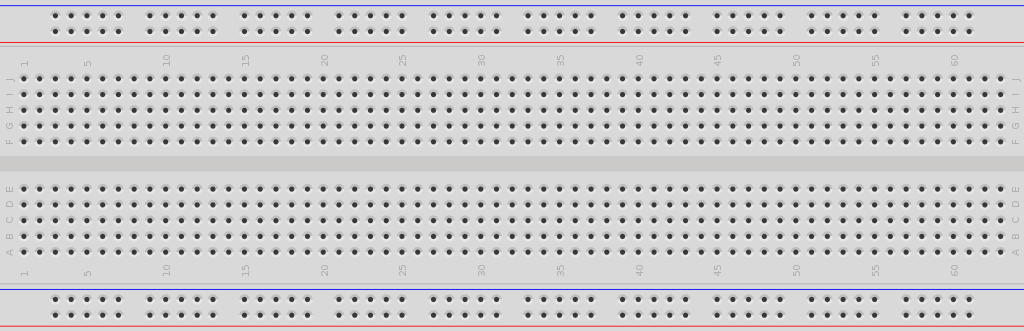
\includegraphics[width=0.8\textwidth]{protoboard_blank}
\caption[An empty prototyping board]{An empty prototyping board.}
\label{fig:protoboard_blank}
\end{figure}

The advantage of a prototyping board is that each of the holes is electrically 
connected to at least four other holes. Thus, by plugging leads wires 
into two connected holes, the leads or wires are now electrically 
connected to each other. The connections in a prototyping board are typically
as follows:
\begin{itemize}
\item All of the holes adjacent to each of the blue lines are connected. 
These are typically used for connections to an electrical ground or the
negative terminal of a power source.
\item All of the holes adjacent to each of the red lines are connected.
These are typically used for connections to an electrical power source 
(generally the positive terminal for DC power sources).
\item Each vertically oriented set of five holes in the center of the board
are connected.
\end{itemize}
These connections are illustrated in Figure \ref{fig:protoboard_connections}.
Please note that not all prototyping boards are alike, and the connections
may vary from board to board.
\begin{figure}[htbp!]
\centering
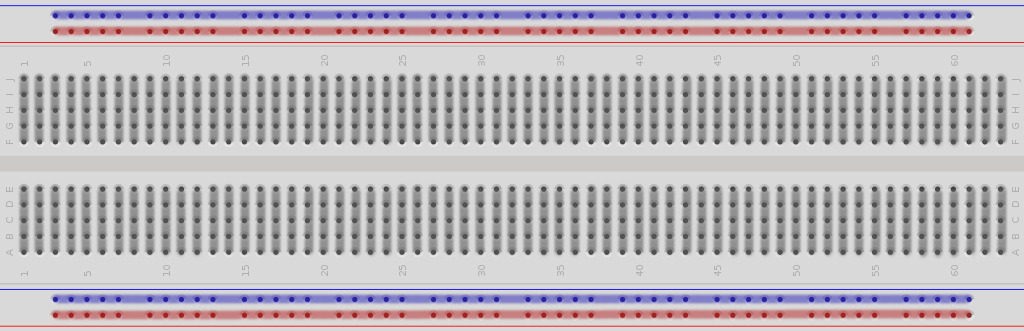
\includegraphics[width=0.8\textwidth]{protoboard_connections}
\caption[Typical connections on a prototyping board]{Typical connections on a
prototyping board. The holes adjacent to each of the red and blue lines are
connected to each other, as indicated by the red and blue highlights on
the figure. The remaining holes are connected in groups of five, as indicated
by the grey highlights.}
\label{fig:protoboard_connections}
\end{figure}

As an example, let's consider how we might wire together a simple circuit 
involving a 9 volt battery and an LED using a protyping board. Note that 
nine volts is usually a little high for powering a single LED, so we are also
going to put a resistor in our circuit to keep the current down.

First, let's connect our battery to the red an blue rows of the 
prototyping board. You don't necessarily have to connect the power this way 
(in fact, once you know how the connections in the prototyping board work, you
can connect things in any fashion consistent with the circuit you are trying 
to build), but doing so is generally considered good practice. We can also
connect each set of row together, so that we are providing a power 
source and ground at both the top and bottom of the board. As you know, the
color of the wires I use doesn't make any difference in how the circuit 
operates, but the colors \textit{can} help me keep track of how I've built my
circuit. Red is typically used for power sources, and dark blue or black is
typically used for ground (or the negative terminal for DC sources). Once I've
made these connections, my prototyping board looks like Figure
\ref{fig:protoboard_example_a}.
\begin{figure}[htbp!]
\centering
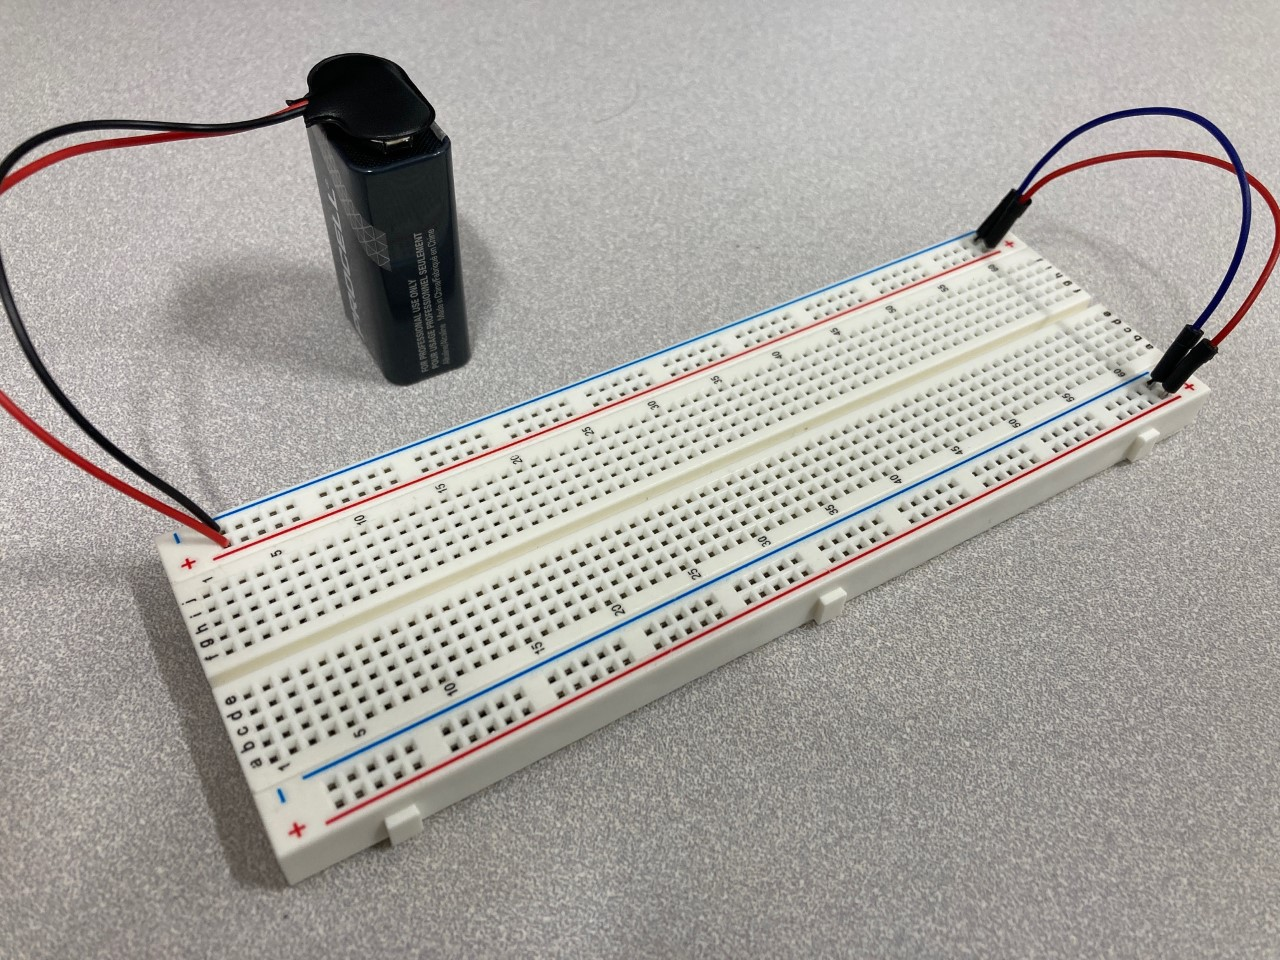
\includegraphics[width=0.8\textwidth]{protoboard_example_a}
\caption[Connecting power to a prototyping board]{Connecting power to a 
prototyping board. Note that the positive lead from the battery holder
connects to the ``red'' horizontal line on the prototyping board, and the
negative lead (the black wire) connects to the ``blue'' line. The red and
blue wires on the right side connect the two red and blue lines together,
respectively.}
\label{fig:protoboard_example_a}
\end{figure}

Our next step is to connect the LED to the red power row. LEDs are picky 
about which lead is connected to power. One of the leads will be longer than the
other. This is the lead that should connect to the power. For our circuit, I 
will plug this long lead directly into one of the holes I've provided power to,
and the other lead into one of the center strips, as seen in Figure
\ref{fig:protoboard_example_b}.
\begin{figure}[htbp!]
\centering
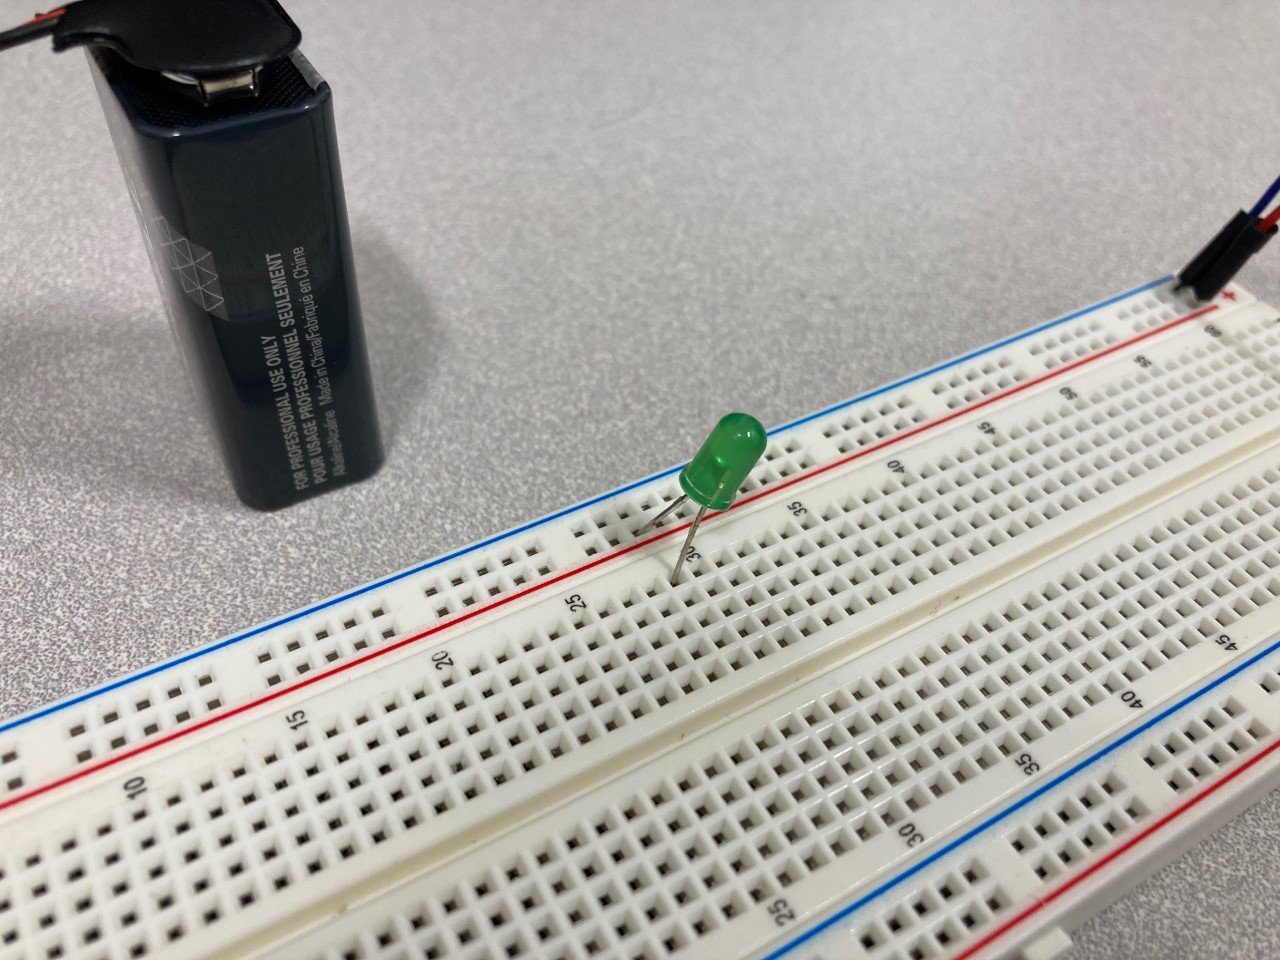
\includegraphics[width=0.8\textwidth]{protoboard_example_b}
\caption[Adding an LED to the prototyping board]{Adding an LED to the 
prototyping board. The long lead is placed in one of the holes connected
to power, and the other lead is connected to a center strip.}
\label{fig:protoboard_example_b}
\end{figure}

At this point, our LED has not lit, because it needs to form a complete circuit,
which we could do by connecting a wire from the unconnected lead to ground
(one of the blue rows). We don't want to do this, though, as the full nine
volts from the battery is probably too much for our LED. So we're going to put
a resistor in first. I'll use a 330 Ohm resistor for this exercise. I connect
one of the resistor leads into the same five hole group that the LED is 
connected to, and the other lead into a hole from a different group (putting
both leads into holes from the same group would be like connecting the two
ends of the resistor together, effectively removing it from the circuit). These
connections can be seen in Figure \ref{fig:protoboard_example_c}.
\begin{figure}[htbp!]
\centering
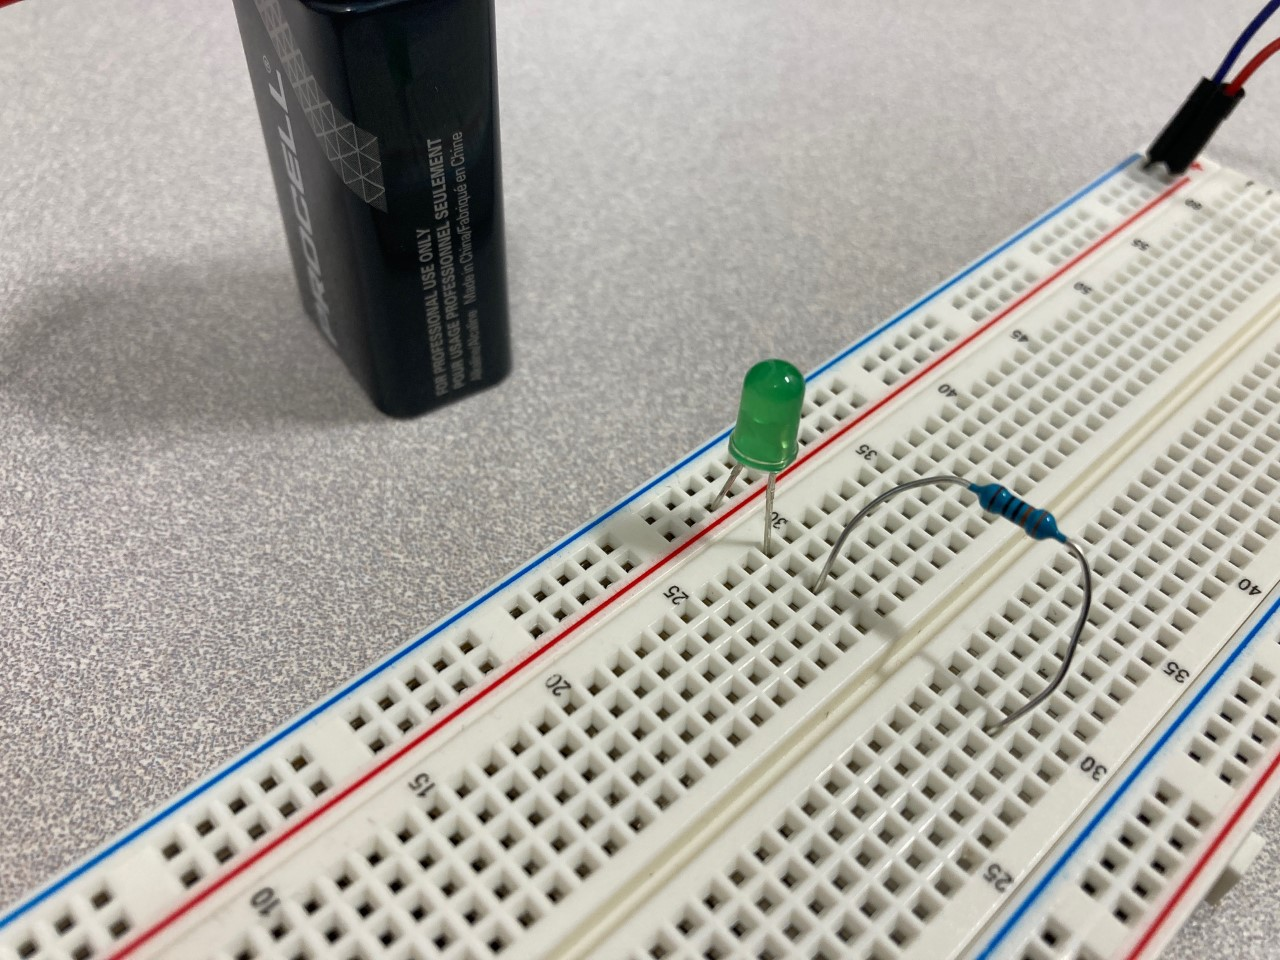
\includegraphics[width=0.8\textwidth]{protoboard_example_c}
\caption[Adding a resistor to the prototyping board]{Adding a resistor to the
prototyping board. One lead is placed in one of the holes in the same group
as the LED lead, and the other lead is connected to a different group.}
\label{fig:protoboard_example_c}
\end{figure}

Our LED is still not lit. We will now complete the circuit by adding a ground
connection. I could have done this by putting the second lead of the resistor
into one of the ground holes, but I'll instead use a wire to finish the
connection. The LED is now lit (Figure \ref{fig:protoboard_example_d})!
\begin{figure}[htbp!]
\centering
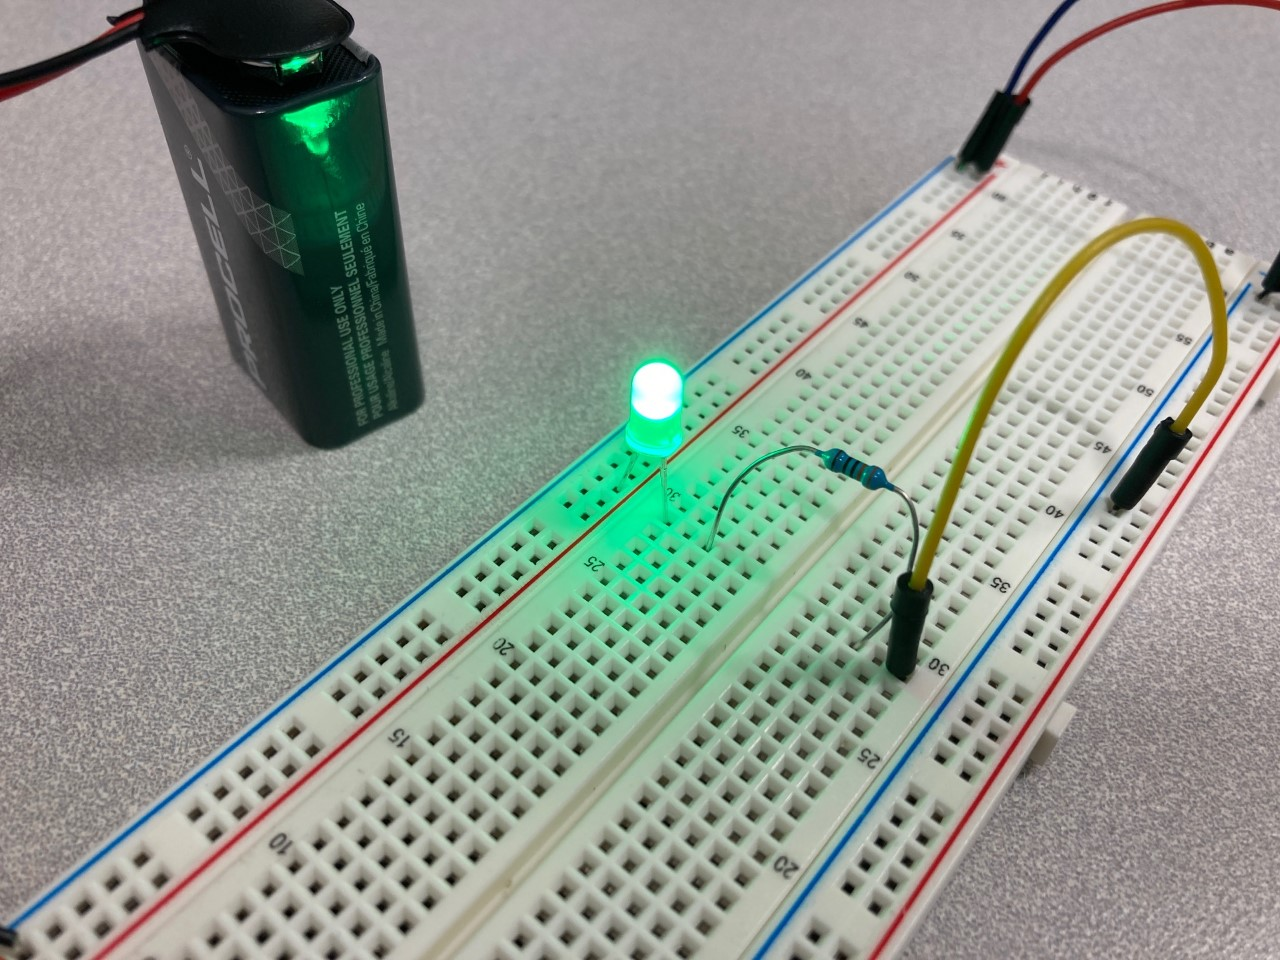
\includegraphics[width=0.8\textwidth]{protoboard_example_d}
\caption[Completing the simple LED circuit]{Completing the simple LED circuit.
One end of the yellow wire is connected to the same group as the end of the
resistor, and the other end of the wire is connected to the ground (blue)
row. Having completed the circuit, the LED is lit.}
\label{fig:protoboard_example_d}
\end{figure}

\activity{
With the exception of the 9 V battery, build the circuit from this example
on a prototyping board.
}

This concludes our example for using a prototyping board to construct a circuit.
Before this lab concludes, we are going to use our Arduino as the power source
for this circuit, and also have a little fun using the Arduino to control the
behavior of the LED. Before we do that, though, we need to talk about soldering.

\subsection{Durable circuits: soldering}

If you followed the last example carefully, you may have 
noted a few things:
\begin{itemize}
\item Using the prototyping board makes this circuit a lot larger than it 
needs to be.
\item We made electrical connections by easily sliding a lead or wire into a
hole. The wire or lead can just as easily be removed from the hole.
\item The entire thing looks like it will fall apart if I try to pick it up
and move it.
\end{itemize}
It is fairly apparent that prototyping boards are good for designing circuits
and building a prototype for testing (hence the name ``prototyping board'').
But if I am going to put this circuit to any sort of practical use, I need to
build it in a more permanent fashion. The way we do this is by electrically
``gluing'' the connections together with solder.

Solder consists of a ductile metal alloy (usually tin, silver, and/or lead) 
mixed with a small amount of material called flux. Solder has a relatively low
melting point, and is also electrically conductive. By melting a little bit of
solder between the wires or leads we want to connect, and then letting the 
solder reset, we can make a mechanically strong connection.

In order to make a mechanically strong and electrically sound connection, 
soldering must be done correctly. The process begins by making sure you have
the right equipment and that it has been properly prepared. Figure
\ref{fig:soldering_equipment} shows the elements of a good soldering station, 
including (from left to right)
\begin{itemize}
\item A soldering iron. This provides the heat to melt the solder.
\item Solder. In this case, it is provided on a spool.
\item Flux paste. Flux is what helps solder flow. Sometimes solder doesn't
have enough flux, and having a little extra paste handy can make a huge 
difference.
\item Tip cleaner. The tip of a soldering iron, after a little use, will start
get gummed up with oxides. When this happens, it doesn't conduct heat very well.
Frequent tip cleaning makes your life a lot easier!
\item Helping hands. This device includes a few clamps that can hold your work
in place, and usually also includes a magnifying glass to help you see what
you are doing. This piece of equipment is critical! Normally, when soldering a
circuit, you need to hold the circuit, the element you are soldering to it, 
the soldering iron, and the solder all at the same time. Unless you have four
hands, you'll need one of these devices!
\item Wire wick. Sometimes you make mistakes while soldering. Wire wick, when 
heated, will sop up solder so you can remove it from your work.
\end{itemize}
\begin{figure}[htbp!]
\centering
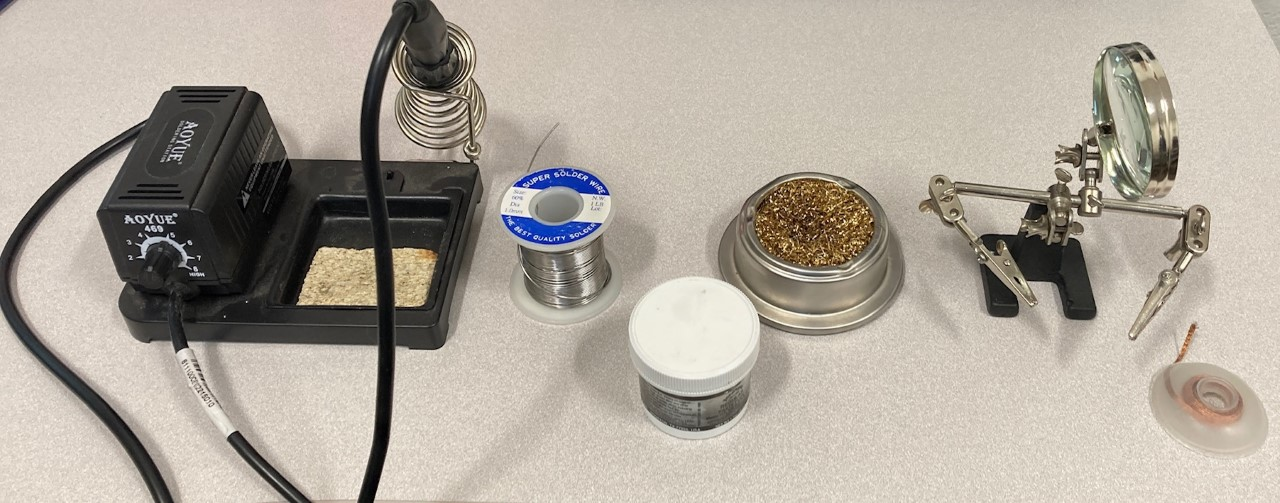
\includegraphics[width=0.8\textwidth]{soldering_equipment}
\caption[Soldering equipment]{Soldering equipment. Included here are
a soldering iron, solder, flux paste, a tip cleaner, a set of ``helping
hands'', and wire wick. See the text for a more full description of these
items.}
\label{fig:soldering_equipment}
\end{figure}

In addition to this equipment, it's also convenient to have a surface to 
solder our components on, rather than trying to solder them together directly.
A common surface is pictured in Figure \ref{fig:perfboard}, and is called a
perfboard. It's basically just a fiberglass board with a bunch of holes
(perforations) drilled in it, and the holes are lined with some sort of 
conductive material.
\begin{figure}[htbp!]
\centering
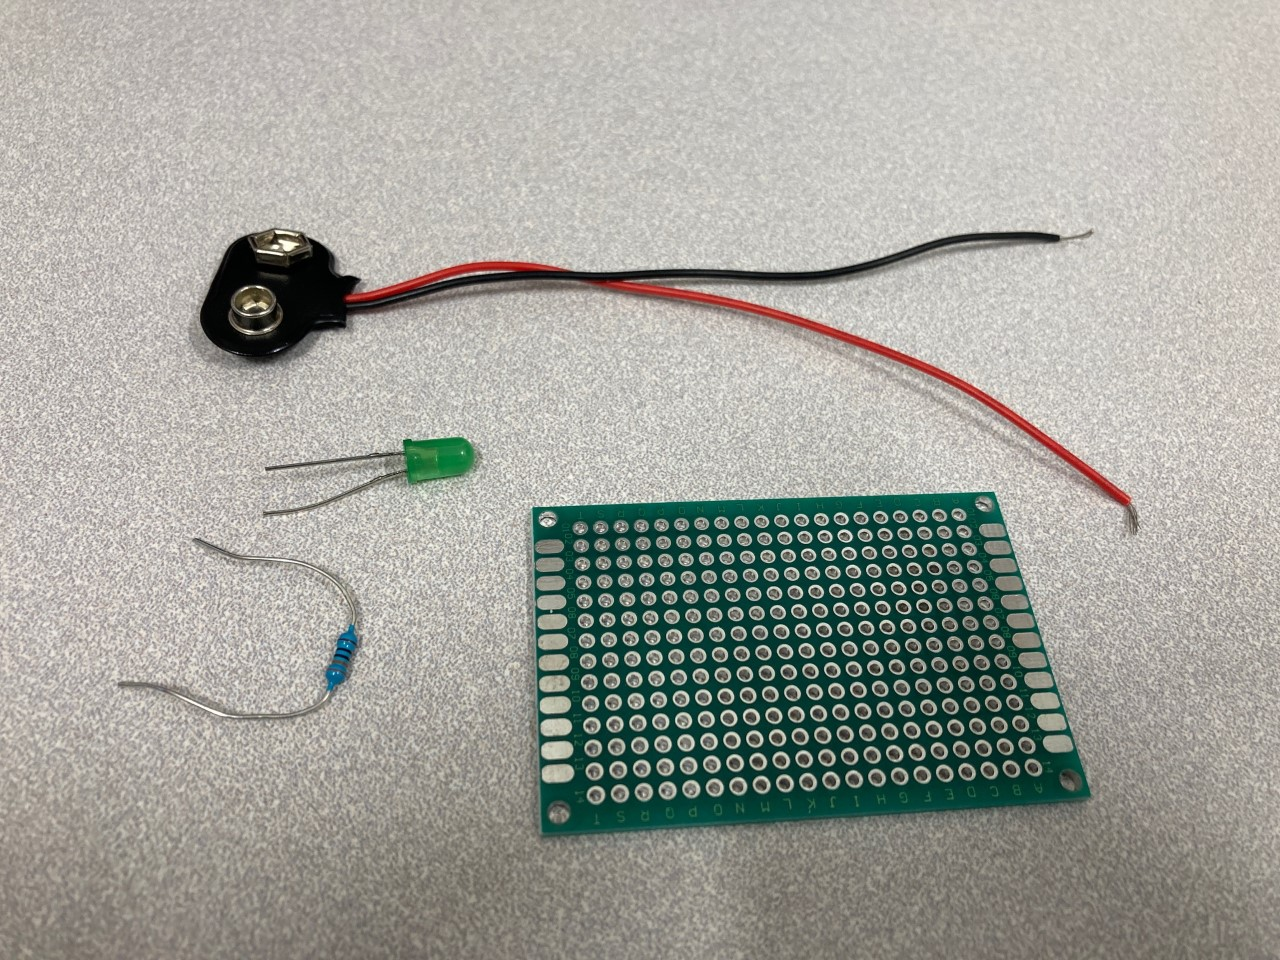
\includegraphics[width=0.8\textwidth]{perfboard}
\caption[A perfboard]{A perfboard, along with some items we will solder
together on it.}
\label{fig:perfboard}
\end{figure}

Now, let's get started. First we'll plug the soldering iron in and give it a 
few minutes to heat up. Once heated, we then want to clean and prepare the tip.
This is done by plunging the tip of the soldering iron in and out of the tip 
cleaner several times. At this point, we'll also dip the tip very briefly 
into the flux paste, and then clean the tip again. Finally, we'll melt a small 
amount of solder onto the tip, and then clean it a third time. At this point,
the tip should be clean and shining with solder, similar to Figure
\ref{fig:solder_ready}.
\begin{figure}[htbp!]
\centering
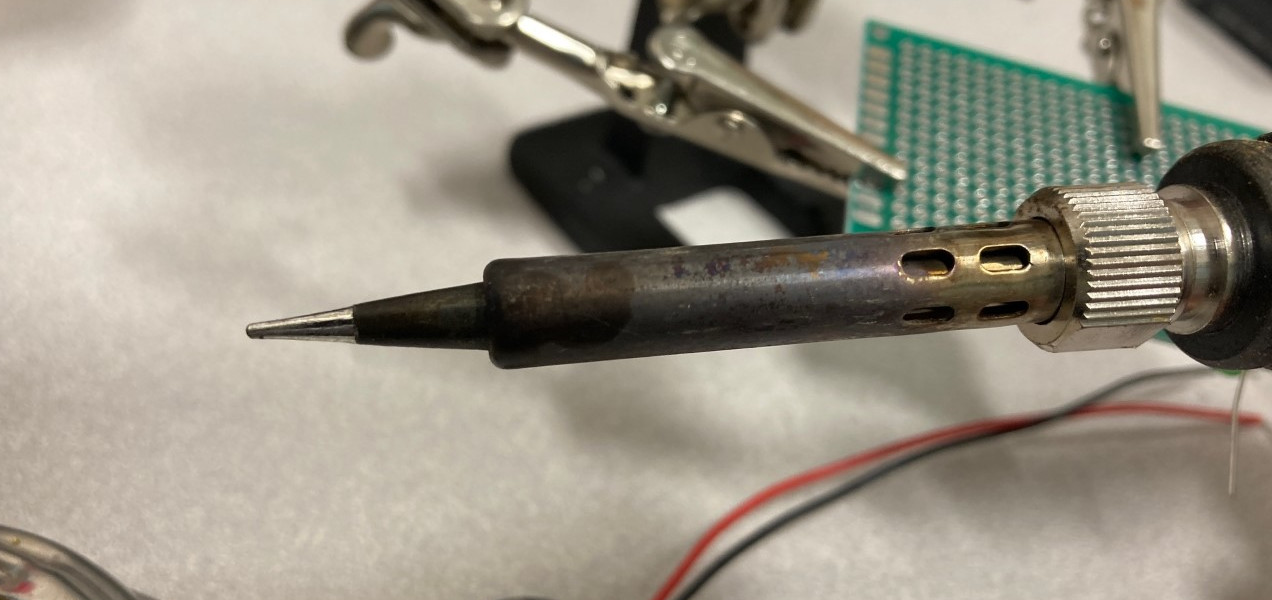
\includegraphics[width=0.8\textwidth]{solder_ready}
\caption[A clean soldering iron tip]{A clean soldering iron tip, ready for
use.}
\label{fig:solder_ready}
\end{figure}

The next step is to start putting elements on the perfboard. Components with
leads can usually be held in place prior to soldering by bending the leads on
the backside of the board. These bent leads can also conveniently be used as
wires between components as well. In Figure \ref{fig:component_preparation},
all of the components for the circuit have been placed on the boards, and 
the leads bent to make electrical connections. Normally you would only add a 
few components at a time, solder those into place, then add more.
\begin{figure}[htbp!]
\centering
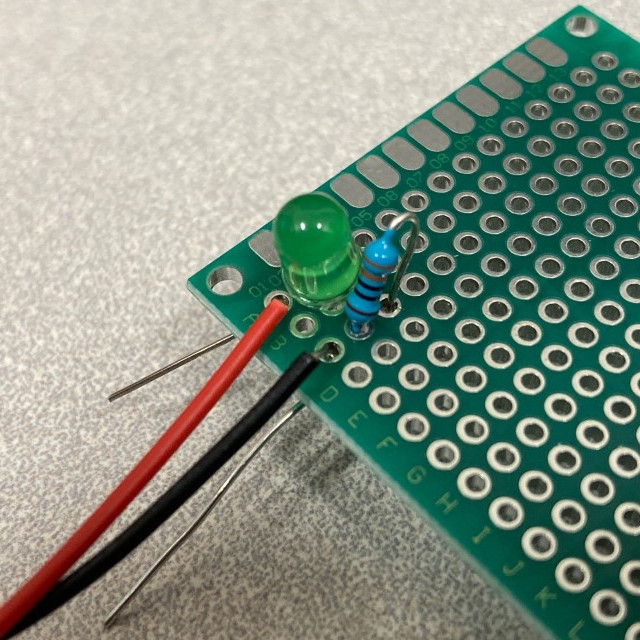
\includegraphics[width=0.4\textwidth]{component_preparation_a}
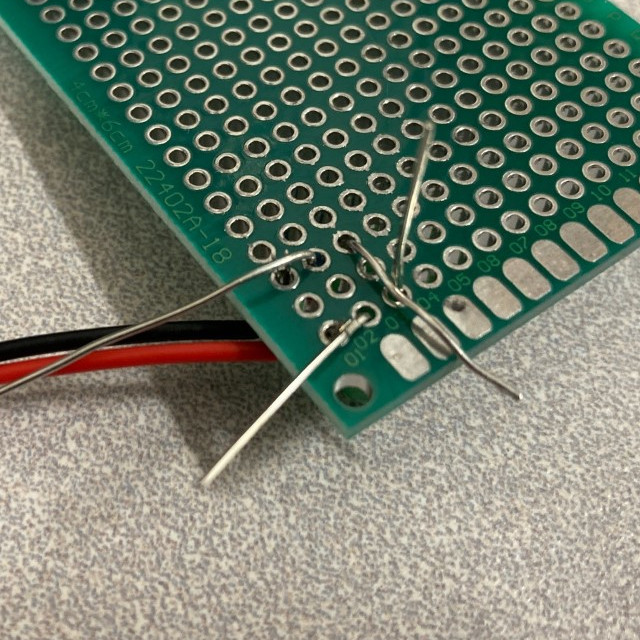
\includegraphics[width=0.4\textwidth]{component_preparation_b}
\caption[Components added to a perfboard, ready for soldering]{Components added
to a perfboard, ready for soldering. Note how, on the back side of the 
perfboard, the leads have been bent to hold the components in place as well as
act as wires.}
\label{fig:component_preparation}
\end{figure}

Now to apply the solder. Rather than trying to hold the entire spool of 
solder, it's easiest to use the soldering iron to burn off a three or so inch
segment instead. A key thing to remember is that you should
\textit{\textbf{heat the work, not the solder}}. If you just touch the solder
with the soldering iron, it will melt, and it might even transfer onto the
parts you are trying to solder. However, the flux tends to move to the 
surface of hot metal, and you'll basically end up with a ball of solder that
is insulated from the work by a thin layer of flux. This is referred to as a
\textit{cold solder} joint, and will likely not provide a lasting electrical
connection. By heating the work and then melting the solder onto the work,
you'll end up with good connections. 
\begin{figure}[htbp!]
\centering
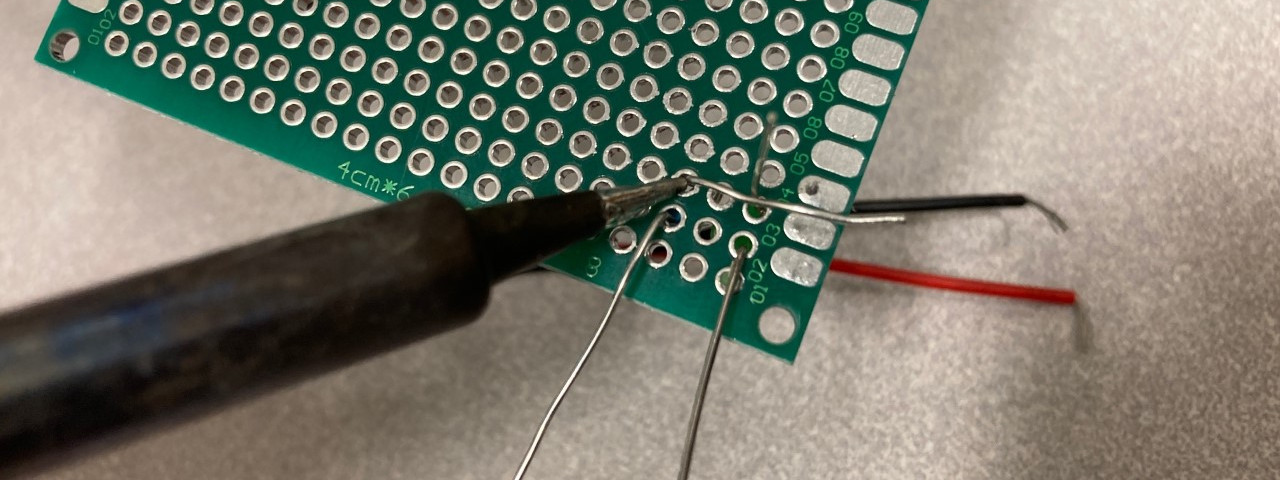
\includegraphics[width=0.8\textwidth]{heat_the_work}
\caption[Heat the work, not the solder!]{Heat the work, not the solder!}
\label{fig:heat_the_work}
\end{figure}

Once the iron is removed from the working area, the solder will cool and set
very quickly.
This process is repeated for each of the
connections. Figure \ref{fig:soldering_almost_done} shows the results with just
a few connections left to solder. In this figure, you'll note that one of the
clamps on the helping hands is holding the wire in place.
\begin{figure}[htbp!]
\centering
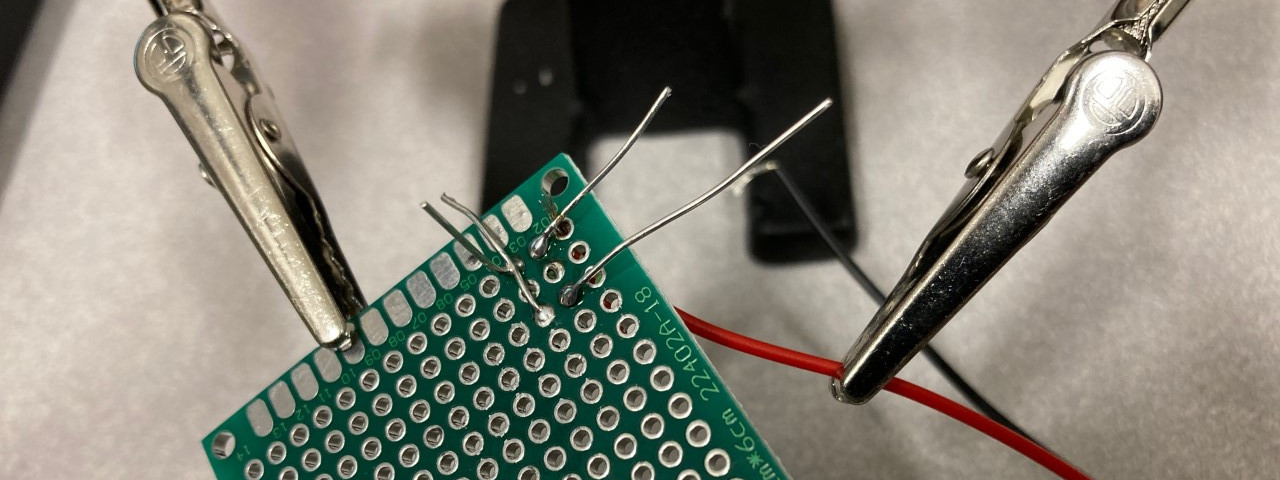
\includegraphics[width=0.8\textwidth]{soldering_almost_done}
\caption[Soldering project near completion]{The soldering project near 
completion. The connections to the 9 V battery connector still need to be
soldered. Note that one of the clamps of the helping hands is holding the red
wire in place.}
\label{fig:soldering_almost_done}
\end{figure}

Once all of the soldering is complete, you'll have some tails of wire and
component lead sticking out. Use a set of close clipping wire cutters to remove
these extra and unnecessary pieces of metal. Now our project is complete
(see Figure \ref{fig:soldering_complete}. Note that the finished product is
significantly more durable than what we had on the prototyping board, and also
significantly smaller. (The perfboard used here is 4 cm by 6 cm, and clearly a much smaller board could have been used.

\begin{figure}[htbp!]
\centering
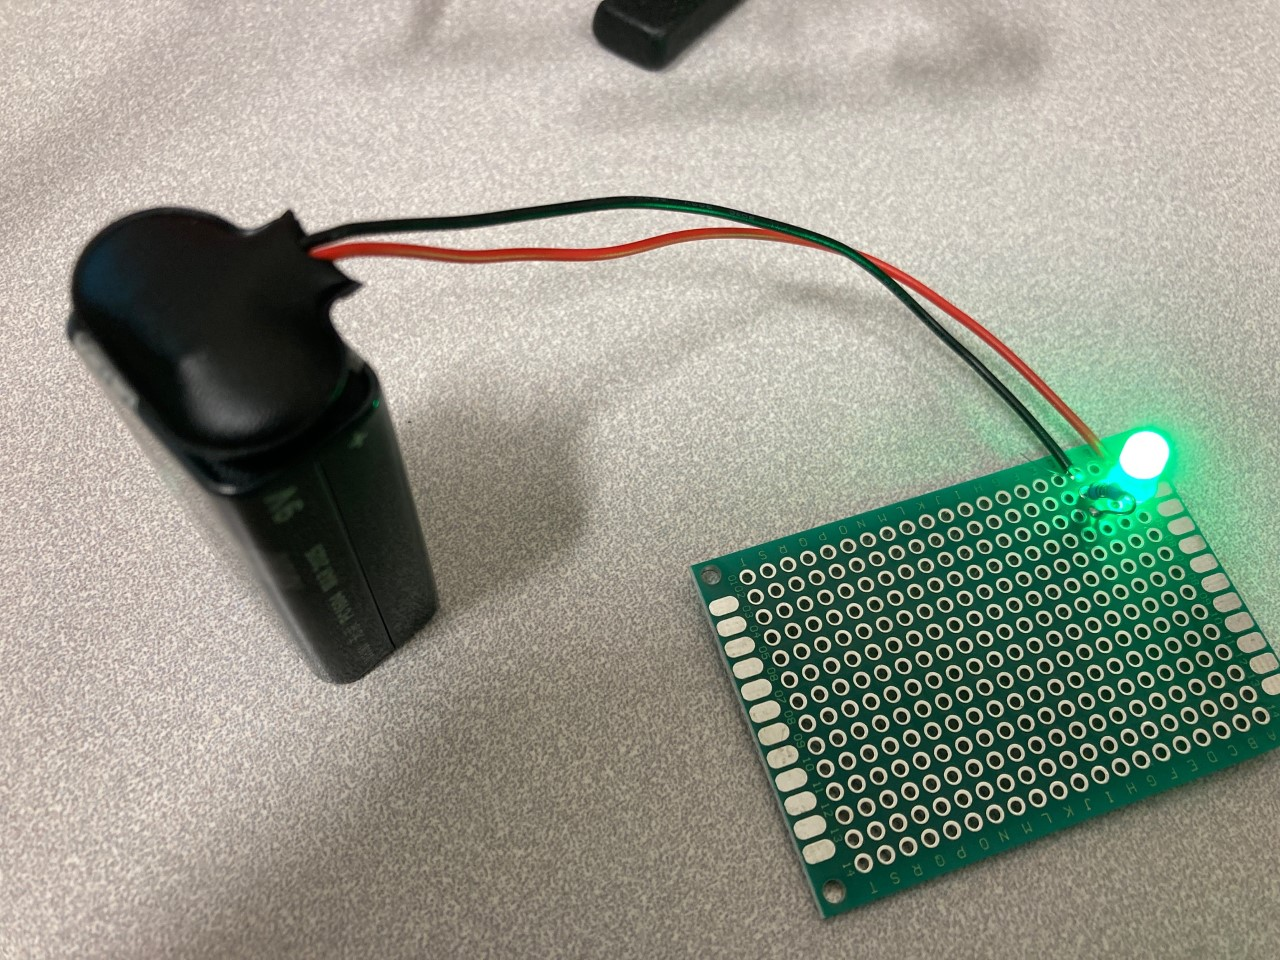
\includegraphics[width=0.8\textwidth]{soldering_complete}
\caption[The completed soldering project]{The completed soldering project.}
\label{fig:soldering_complete}
\end{figure}

\activity{
Successfully complete three or more soldering connections.
}

Now that we've seen how to design, build, and solder circuits, let's look at
controlling our circuit using an Arduino.

%%%%%%%%%%%%%%%%%%%%%%%%%%%%%%%%%%%%%%%%%%%%%%%%%%%%%%%%%%%%%%%%%%%%%%%%%%%%%%%%

\section{Arduino Circuit Control}

Let's start our study of computer control by controlling something simple
with an Arduino DAQ: the LED circuit that we constructed earlier on the
prototyping board. Our objective is to use the Arduino to turn the LED on and 
off. 

\subsection{Attaching the Arduino to the circuit}

\subsection{The Arduino sketch: an introduction}

\subsection{Compiling and uploading the sketch}

%\begin{figure}[h!]
%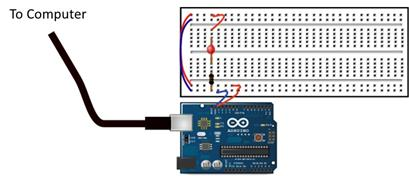
\includegraphics[width=3.4504in,height=1.4955in]{PH4CAU01}
%\end{figure}

%Let's assemble our system one step at a time.


%Now we can wire our light to our Arduino. This will take two wires. One
%should be wired to pin13. The pin numbers are given on the side of the
%wiring areas. \begin{figure}[h!]
%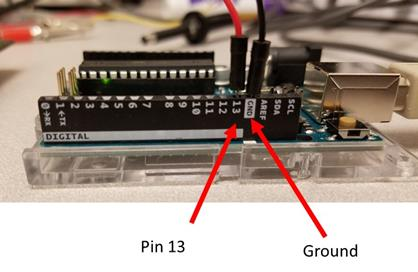
\includegraphics[width=3.5258in,height=2.3017in]{PH4CAU0B}
%\end{figure}This pin 13 is a digital output.
%That means it will either have $5\unit{V}$ or it will have $0\unit{V}.$ The $%
%5\unit{V}$ will be our \textquotedblleft on\textquotedblright\ value that
%could turn on an instrument. In our case it will turn on our LED\ light. The 
%$0\unit{V}$ is the \textquotedblleft off\textquotedblright\ value. When pin
%13 has a value of $0\unit{V}$ our light will go off. We know that voltage is
%related to electrical energy. We will study voltage more next week. But for
%now we need to know that voltage is a comparison. So we need to know
%\textquotedblleft $5\unit{V}$ compared to what?\textquotedblright\ We
%compare to the voltage of the ground. This is literal. Most buildings have a
%large copper rod pounded into the ground. All of the plugs in the building
%have one of their three wires connected to this rod. Thus they are all
%\textquotedblleft grounded.\textquotedblright\ This is our reference. Our
%computer is connected to a plug so it is grounded. Our Arduino is connected
%to the computer so it is grounded. And one of our pins is a connection to
%the ground. It is marked \textquotedblleft GND.\textquotedblright\ This will
%be our $0\unit{V}.$ So we need to connect pin 13 and the GND pin to our $+5%
%\unit{V}$ and our $0\unit{V}$ rows on our proto-board. The next figure shows
%one way to do this.

%\begin{figure}[h!]
%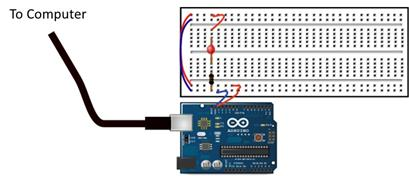
\includegraphics[width=3.4504in,height=1.4955in]{PH4CAU0C}
%\end{figure}

%We now have hour \textquotedblleft hardware\textquotedblright\ built for
%blinking a light. But we need to give instructions to our Arduino that tells
%it what to do with pin 13 and pin GND so our light will blink. Our Arduino
%has a small computer on board, and we need a computer program to be uploaded
%to the Arduino for this small computer to run. We will write and upload that
%program next.

%\subsection{LED light blink Sketch}

%You wrote computer programs in Python in PH150. Our Arduino programs are
%similar. They have loops and mathematical statements. There are some
%differences as well. Our Arduino programs have special code
%\textquotedblleft objects\textquotedblright\ for controlling our Arduino.
%Most Arduino programs are very short. We just need instructions to tell the
%Arduino what to turn on, turn off, or what data to collect. For today's lab,
%we just need to address the digital output pins.

%Let me introduce the commands we will use. Each digital output has a number.
%The code defines a variable of type integer (int) and sets it equal to the
%pin number. That pin can be HIGH or LOW with HIGH $=+5\unit{V}$ and LOW $=0%
%\unit{V}$. Each digital pin needs to be set up for output or input. This is
%done with a pinMode statement:

%\begin{equation*}
%\begin{tabular}{l}
%pinMode(ledPin, OUTPUT)%
%\end{tabular}%
%\end{equation*}%
%The variable ledPin is the pin number (for us 13). And the key word
%\textquotedblleft OUTPUT\textquotedblright\ sets up our pin 13 to turn
%things on or off.

%To set the pin to HIGH use a digitalWrite command

%\begin{equation*}
%\begin{tabular}{l}
%digitalWrite(ledPin,HIGH);%
%\end{tabular}%
%\end{equation*}%
%and finally, to let the light be on for a while, use a delay command where
%the delay time is given in milliseconds (ms)%
%\begin{equation*}
%\begin{tabular}{l}
%delay(100);%
%\end{tabular}%
%\end{equation*}

%These would not be normal Python commands. They are part of a specific code
%library for use in making things with Arduino's.

%We have a special development environment for programing our Arduino as
%well. It looks like this. \begin{figure}[h!]
%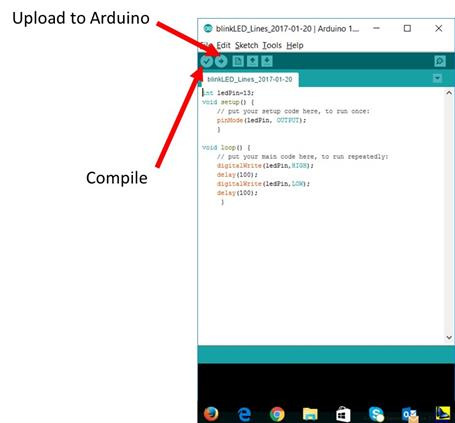
\includegraphics[width=3.8353in,height=3.5674in]{PH4CAU0D}
%\end{figure}We will need to install this
%development environment. To do so we go to
%https://www.arduino.cc/en/Guide/HomePage and choose to instal the Arduino
%IDE for your computer. IDE stands for \textquotedblleft integrated
%development environment.\textquotedblright\ This is the environment that you
%see in the last figure. It has two unusual buttons on its toolbar. One is
%the \textquotedblleft compile\textquotedblright\ button. When you used
%Python in PH150, you could run your code by pushing on a green arrow button
%in most development environments. If you used Jupyter scripts, they also had
%a function to run your code. But our Arduino is not big enough to be able to
%run code this way. We need to convert our human-understandable code that
%looks mostly like Python into a digital format that the Arduino can
%understand. The compile button does this. As the code is converted, the
%Arduino software looks for errors in the code. If there are errors, it will
%tell you at this point. This is different than Python which only told you
%about errors as the code ran. But remember we don't want to run our program
%on our computer. We want it to run on our Arduino. So this check is good
%before we send the translated code to the Arduino.

%We also need a way to send our code to our Arduino and that is what the
%upload to Arduino button does. Once the code is compiled without errors,
%connect the USB\ cable to the Arduino and push the upload button.

%There are also some syntax differences between the Arduino computer language
%and Python. If you have taken CS124 or know the \textquotedblleft
%C\textquotedblright\ language, you will recognize some of these changes.

%\begin{itemize}
%\item Everything in a function needs to be in curly braces \{ \}

%\item Indenting is a good idea, but not required

%\item comments can be started with two slashes //

%\item every line needs a semicolon at the end;
%\end{itemize}

%\subsection{Arduino LED light blink sketch (program)}

%We are ready to write code to blink our LED\ light. Here is an example code.
%We write this code right in the Arduino development environment main window. You can download it directly \href{https://dtoliphant.github.io/PH250Manual/Code/IntroBlink.ino}{here}
%\lstinputlisting[language=Arduino]{Code/IntroBlink.ino}


%%\begin{lstlisting}[language=Arduino]
%%/////////////////////////////////////////////////////////
%%//Arduino Sketch to blink one LED light
%%//   Written by Brother Lines
%%//	(place your name here in your code)
%%//   Feb 6, 2017
%%//
%%//   Define our Arduino Variables
%%//      We will call pin 13 "ledPin"
%%/////////////////////////////////////////////////////////
%%int ledPin=13;
%% 
%%/////////////////////////////////////////////////////////
%%// Arduino setup function comes next
%%//    Every Arduino sketch needs a setup function
%%//    We will set up our ledPin (pin 13) as an output pin
%%void setup() {
%% // put your setup code here, to run once to set up:
%% pinMode(ledPin, OUTPUT);
%% }
%% 
%%/////////////////////////////////////////////////////////
%%// Arduino loop function
%%//    Every Arduino sketch has a loop function
%%//    This is where we put what we want the Arduino to do
%%//    The Arduino will do whatever is in the loop function 
%%//    until the Arduino is unplugged.
%% 
%%void loop() {
%% // put your main code here, to run repeatedly:
%% // turn on the LED
%% digitalWrite(ledPin,HIGH);
%% 
%% // leave in on for 100ms
%% delay(100);
%% 
%% // turn off the LED
%% digitalWrite(ledPin,LOW);
%% 
%% // leave in off for 100ms
%% delay(100);
%% }
%%/////////////////////////////////////////////////////////
%%/////////////////////////////////////////////////////////
%%\end{lstlisting}

%Notice that we used a lot of comments. There are only ten lines that are
%actually required to make the sketch run.

%\begin{lstlisting}[language=Arduino] 
%int ledPin=13;
%void setup() {
% pinMode(ledPin, OUTPUT);
% }
%void loop() {
% digitalWrite(ledPin,HIGH);
% delay(100);
% digitalWrite(ledPin,LOW);
% delay(100);
% }
% 
%\end{lstlisting}

%The comments are not required for the sketch to work, but they help us
%remember what we did later. In our class, \textbf{comments are required for
%full credit}. So don't leave out the comments. In fact, you can add any
%comments that might help you remember why the code works.

%Also notice that Arduino programs are called \textquotedblleft
%sketches.\textquotedblright\ Most of the commands are special Arduino
%commands. And luckily, they make sense when we read them. Try it out. Type
%in this sketch including the comments and compile and upload it to your
%Arduino. If all goes well, the LED light will begin to blink. If all did go
%well, go on to the next section. If it did not, call over an instructor.

%Save your sketch and maybe take a photo of your hardware set up. Place both
%in your lab notebook along with notes on how you got it to work. We will
%build on this sketch, so spend some time documenting what you did in your
%lab notebook so you can refer to it later.

\activity{
Build your own clone of the blinking light circuit described in this section
by doing each of the following:
\begin{itemize}
\item Construct the LED circuit on a prototyping board.
\item Connect the Arduino to the LED circuit and to your computer.
\item Write, compile, and upload the sketch to the Arduino.
\item Verify that the circuit is working correctly.
\end{itemize}
}

%%%%%%%%%%%%%%%%%%%%%%%%%%%%%%%%%%%%%%%%%%%%%%%%%%%%%%%%%%%%%%%%%%%%%%%%%%%%%%%%

\section{Adding More Complexity}



%Now let's see if we can apply what we have learned. Let's change our
%hardware so that it has two LED lights. Most of the hardware setup will be
%the same. But We will wire them to two Arduino pins, say 12 and 13 (along
%with GND of course) and have them blink, but blink independently.

%We will have to abandon our nice $+5\unit{V}$ top row as our connection to
%pin 13 because we need two pins, 12 and 13. The two pins must work
%independently. In fact, let's have one LED\ on when the other is off.

%This is why we can't wire both LED lights to the top row and wire the top
%row to pin 13 as we did last time. That would make both lights blink at
%once, but would not let one be off and the other on. Instead, let's wire the
%top lead of one LED directly to pin 13 of our Arduino, and let's wire the
%top lead of the other LED to pin 12. The two resistors can share a
%connection to the GND pin, so let's keep using the $0\unit{V}$ bottom row of
%the proto-board. Your hardware should look something like this.

%\begin{figure}[h!]
%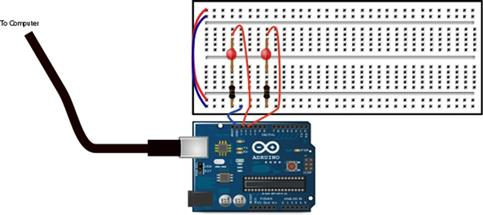
\includegraphics[width=4.0704in,height=1.8228in]{PH4CAU0E}
%\end{figure}We will need to modify our sketch
%(save the old one first so you have a separate copy for reference). Here is
%a suggestion of what the new sketch might look like.

%\lstinputlisting[language=Arduino]{Code/IntroBlink2LEDs.ino}


%Again save your sketch and maybe take a photo of your hardware set up. Place
%both in your lab notebook along with notes on how you got it to work. Make
%sure others at your table are able to get their setup to work.

\activity{
Using the Arduino and prototyping board, construct a circuit with all of the 
following characteristics:
\begin{itemize}
\item Increments a counter every half second.
\item Turns on a red LED only when the counter is an even number.
\item Turns on a yellow LED only when the counter is a multiple of three.
\item Turns on a green LED only when the counter is a multiple of five.
\item Turns on a blue LED only when the counter is a multiple of seven.
\end{itemize}
}

% NOTE: In previous versions of the textbook, two additional activities were 
% included in which the students would make the light blink in a Fibonacci 
% sequence. One author (Kevin) noted that, since the students were just
% copy/pasting the code, they weren't getting a whole lot from this, other
% than noting that the Arduino can do math. I've included some additional
% processing in the previous activity. Additionally, because I've now included
% the section and activity on soldering, they may not have sufficient time to
% do these last activities. Hence, I have excluded them from this version.
% However, the original code is included below.

% \section{Third Computer Control: Two LED blink using math}

% Let's leave our hardware alone in the two LED setup from the last section.
% And let's make the LED's blink the same way. But this time, let's calculate
% when they should be on or off. Why would we do this? Because sometimes in
% computer control of experiments we need to turn something on or off based on
% a calculation. You may have your computer watching to make sure the
% experiment doesn't get too hot or cold. The Arduino can bring in temperature
% information, but you would have to write the code to tell it to turn off the
% heater when your experiments gets to hot and to turn it on when it gets too
% cold. This could be done with a mathematical comparison. We will use such a
% comparison in the next sketch.

% Suppose we want to know if a number is even or odd. Even numbers are evenly
% divisible by $2.$ We could divide a number by $2$ and see if the remainder
% is zero. Our Arduino language has a good set of mathematical functions. The
% remainder function is a \textquotedblleft \%\textquotedblright\ sign. For
% example 
% \begin{eqnarray*}
% 3\%2 &=&1 \\
% 6\%2 &=&0
% \end{eqnarray*}%
% Let's have one light turn on if a number is even, then switch to the other
% light if the number is odd.

% In our code we will introduce a variable, $i,$ that we will increment (add
% one to) every time the loop runs. So the first time the Arduino loop runs it
% will be zero (even) and the next time 1 (odd) and the next time 2 (even) and
% the next time 3 (odd) and so on. If you studied Python you would call such a
% variable an \textquotedblleft integer\textquotedblright\ and might even know
% to call it a \textquotedblleft loop counter.\textquotedblright

% In our Arduino sketch we will test to see if $i$ is even in an if-statement.
% If-statements go like this
%  \begin{lstlisting}[language=Arduino]
%  if (test condition ) {
%    do something;
%  }
%  else {
%    do something else;
%  }
%  \end{lstlisting}

% Notice that the parts of the if-statement need curly braces. Our condition
% to test is
%  \begin{lstlisting}[language=Arduino]
% i % 2 == 0
%  \end{lstlisting}

% Note that there are two equals signs. That makes it a test for equality
% rather than an assignment. So we will have an if-statement like this
%  \begin{lstlisting}[language=Arduino]
% if (i % 2 == 0 ) {
%  digitalWrite(ledPin1,HIGH);
%  digitalWrite(ledPin2,LOW);
%  delay(1000);
%  }
%  else {
%  digitalWrite(ledPin1,LOW);
%  digitalWrite(ledPin2,HIGH);
%  delay(1000);
%  }
%  
%  \end{lstlisting}

% One last addition, our Arduino language has a shortcut for the statement
%  \begin{lstlisting}[language=Arduino]
% i=i+1
%  \end{lstlisting}

% It is simply
%  \begin{lstlisting}[language=Arduino]
% i++
%  \end{lstlisting}

% We will use this to make $i$ increase by one each time the loop runs. The
% whole code might look like this.
% \lstinputlisting[language=Arduino]{Code/IntroBlink2LEDs_Math.ino}



% Again save your sketch. You should probably say in your lab notebook that
% you used the previous hardware setup. You might want to describe in your lab
% notebook how the mathematical algorithm works.

% \section{Fourth Computer Control: Two LED blink in the Fibonacci sequence}

% Suppose instead of LED\ lights we had large radio transmitters. And suppose
% we were part of the Search for Extra-Terrestrial Intelligence (SETI). We
% wish to send a message to any intelligent life that they would understand.
% Intelligent life probably would be able to do mathematics and would
% understand how mathematics occurs in nature. One sequence of numbers that
% occurs over and over again in nature was discovered by Fibonacci. Let's
% blink our LED\ lights (representing those powerful radio transmitters) in
% the Fibonacci sequence.

% We need to know now to calculate the Fibonacci sequence. One method is to
% know that the sequence goes like this%
% \begin{equation*}
% 0,1,1,2,3,5,8\ldots
% \end{equation*}%
% and that we can find the next number in the sequence by choosing $f_{1}=0$
% first, then $f_{2}=1$ then using the formula 
% \begin{equation*}
% f(x-1)\ +\ f(x-2)
% \end{equation*}%
% Let's see that this works. For the first of the sequence, we just write the $%
% 0.$ For the second we just write the $1.$ Then for the third 
% \begin{eqnarray*}
% f_{3} &=&f_{2}+f_{1} \\
% &=&1+0 \\
% &=&1
% \end{eqnarray*}%
% So far so good. Let's try the next in the sequence%
% \begin{eqnarray*}
% f_{4} &=&f_{3}+f_{2} \\
% &=&1+1 \\
% &=&2
% \end{eqnarray*}%
% Again it worked. For the next one%
% \begin{eqnarray*}
% f_{5} &=&f_{4}+f_{3} \\
% &=&2+1 \\
% &=&3
% \end{eqnarray*}%
% and though we won't prove it, it works for every member of the sequence. See
% if you can figure out how to write this code. An example is given below, but
% see if you can figure out what the code should be.

% This example is a much more complex version of a mathematical based computer
% control.
% \lstinputlisting[language=Arduino]{Code/IntroFibonacci.ino}
% % \begin{lstlisting}[language=Arduino]
% %/////////////////////////////////////////////////////////
% %// code to blink two LED's using a mathematical expression
% %// to determine when they should light. Note that the
% %// Arduino code is closer to C++ than python.
% %/////////////////////////////////////////////////////////
% %int ledPin1=13;
% %int ledPin2=12;
% %int i=0; //loop counter
% % 
% %/////////////////////////////////////////////////////////
% %int fib_count=0; // number of blinks based on Fibonacci
% %int i_max=10; // maximum Fibonacci number before 
% % // starting over
% % 
% %/////////////////////////////////////////////////////////
% %void setup() {
% % // put your setup code here, to run once:
% % pinMode(ledPin1, OUTPUT);
% % pinMode(ledPin2, OUTPUT);
% % } 
% % 
% %int fib(int x) {
% % // calculates the Fibonacci sequence using recursion
% % if (x==0) 
% %    return 0;
% % if (x==1)
% %   return 1;
% %   return fib(x-1) + fib(x-2);
% % } 
% % 
% %/////////////////////////////////////////////////////////
% %void loop() {
% % // put your main code here, to run repeatedly:
% % // blink the LED's with the number of blinks being 
% % // the Fibonacci sequence.
% % fib_count=fib(i);
% % if (i % 2 == 0 ) {
% %   // turn off one light
% %   digitalWrite(ledPin2,LOW);
% %   // now blink the second light fib_count times 
% %   for (int n=0; n<fib_count; n++) { 
% %      digitalWrite(ledPin1,HIGH);
% %      delay(100);
% %      digitalWrite(ledPin1,LOW);
% %      delay(100);
% %   }
% % }
% % else {
% %   // turn off the other light
% %   digitalWrite(ledPin1,LOW);
% %   // now blink the first light fib_count times
% %   for (int n=0; n<fib_count ; n++) { 
% %      digitalWrite(ledPin2,HIGH);
% %      delay(100);
% %      digitalWrite(ledPin2,LOW);
% %      delay(100);
% %   }
% % }
% % // increment i
% % i++;
% % // limit our blinks to the first i_max Fibonacci numbers
% % if (i>i_max) i=0;
% % }
% %}
% %/////////////////////////////////////////////////////////
% %/////////////////////////////////////////////////////////
% % \end{lstlisting}

% Again save your sketch. You should probably say in your lab notebook that
% you used the previous hardware setup. You really should describe in your lab
% notebook how the mathematical algorithm works.

% For next week, you should read the lab before coming to class. So your
% assignment is to read Lab 2.

% %TCIMACRO{\TeXButton{\vspace*{\fill}}{\vspace*{\fill}}}%
% %BeginExpansion
% \vspace*{\fill}%
% %EndExpansion
% \pagebreak
